% ACM DL Format
\documentclass[sigconf]{acmart}

% Paquetes necesarios
\usepackage[utf8]{inputenc}
\usepackage[spanish]{babel}
\let\Bbbk\relax
\usepackage{amsmath,amssymb,amsfonts}
\usepackage{algorithmic}
\usepackage{graphicx}
\usepackage{textcomp}
\usepackage{xcolor}
\usepackage{float}
\usepackage{caption}
\usepackage{booktabs}

% Cambiar "Figura" por "Fig." y ajustar formato
\addto\captionsspanish{\renewcommand{\figurename}{Fig.}}
\captionsetup[figure]{labelformat=simple, labelsep=period, name=Fig., labelfont=bf}

% Información del copyright ACM (ajustar según corresponda)
\copyrightyear{2026}
\acmYear{2026}
\setcopyright{acmlicensed}

\begin{document}
\renewcommand{\abstractname}{Abstract}

% Título del artículo
\title[IPS for DoS Mitigation in ICS]{Implementation of an Intrusion Prevention System for Mitigating DoS Attacks in Industrial Control Networks Based on PLC and Industrial Switch Protection}

% Sobreescribir manualmente el encabezado de autores
%\renewcommand{\shortauthors}{Juarez Mayo et al.}

% Autores y afiliaciones
\author[ ]{Manuel Oswaldo Juarez Mayo}
\affiliation{%
  \institution{Universidad Nacional de Trujillo}
  \country{Peru}
}
\email{t1022701121@unitru.edu.pe}

\author[ ]{Jose Alfredo Valdez Reyes}
\affiliation{%
  \institution{Universidad Nacional de Trujillo}
  \country{Peru}
}
\email{t1052702321@unitru.edu.pe}

\author[ ]{Alberth Jesus Vigo Saldaña}
\affiliation{%
  \institution{Universidad Nacional de Trujillo}
  \country{Peru}
}
\email{t1022700221@unitru.edu.pe}

\author[ ]{Javier Eduardo Villegas Vidal}
\affiliation{%
  \institution{Universidad Nacional de Trujillo}
  \country{Peru}
}
\email{t1512700721@unitru.edu.pe}

\author[Juarez Mayo et al.]{Jesús Moises Martin Villar Castillo}
\affiliation{%
  \institution{Universidad Nacional de Trujillo}
  \country{Peru}
}
\email{t052700420@unitru.edu.pe}

\begin{abstract}
Industrial Control Systems (ICS) are increasingly exposed to cyberattacks due to the integration of operational technology (OT) with IP-based networks. Among these threats, Denial-of-Service (DoS) attacks critically affect process availability by targeting Programmable Logic Controllers (PLCs) and industrial switches. This study presents the design and implementation of an Intrusion Prevention System (IPS) architecture to mitigate DoS attacks in industrial control networks. The experimental setup used a virtual environment with OpenPLC controllers, SCADA components, and IPS tools (Suricata) to evaluate performance under SYN, ICMP, UDP, and Modbus TCP flooding. Results show that IPS deployment effectively reduced latency, packet loss, and service interruptions while maintaining PLC availability and stable communication. The proposed architecture strengthened the resilience of the industrial network against DoS threats.
\end{abstract}

\keywords{Industrial Control Systems, Intrusion Prevention System, DoS Mitigation, PLC Protection, SCADA Networks, Cybersecurity}

\maketitle

\section{Introduction}
Industrial Control Systems (ICS) constitute the technological foundation of critical infrastructures such as energy, manufacturing, transportation, water treatment, and industrial automation environments. The rapid integration of Operational Technology (OT) with Information Technology (IT) and Industrial Internet of Things (IIoT) architectures has significantly improved industrial connectivity and operational efficiency. However, this convergence has also increased the exposure of industrial environments to sophisticated cyber threats targeting communication networks, industrial devices, and supervisory systems.

Modern ICS environments commonly incorporate Ethernet-based communication technologies and TCP/IP industrial protocols that facilitate remote access and interoperability but simultaneously introduce new cybersecurity vulnerabilities \cite{Gillen2020ICS}, \cite{Tama2022IDS}.

Among the most critical threats affecting industrial environments are Denial-of-Service (DoS) attacks, which aim to disrupt the availability of industrial services and communication infrastructures by overwhelming network resources or industrial devices with malicious traffic. In industrial contexts, the interruption of communication between Programmable Logic Controllers (PLCs) \cite{Raman2021ICS}, Human Machine Interfaces (HMIs), and SCADA systems may produce operational instability, process interruption, safety risks, and economic losses. Unlike conventional IT systems, industrial networks require high availability, deterministic communication, and real-time responsiveness, making them particularly vulnerable to traffic flooding attacks and resource exhaustion scenarios \cite{Benka2025ICS}.

According to Yu et al. \cite{Yu2019Ethernet}, Programmable Logic Controllers (PLCs) represent one of the most critical components within industrial control architectures because they directly interact with physical processes and industrial equipment. Nevertheless, many PLCs were originally designed prioritizing operational reliability rather than cybersecurity protection, resulting in limited authentication mechanisms, insufficient encryption capabilities, and weak resistance against network-based attacks. Similarly, industrial communication protocols such as Modbus/TCP, Profinet, and EtherNet/IP were initially developed without integrated security mechanisms, facilitating malicious traffic injection, unauthorized access, and denial-of-service exploitation \cite{Modbus2025IDS}.

According to Tama et al. \cite{Tama2022IDS}, Intrusion Prevention Systems (IPS) have emerged as an effective security mechanism capable of detecting and blocking malicious network activities in real time. IPS technologies combine traffic inspection, signature-based detection, anomaly analysis, and automated response mechanisms to prevent cyberattacks before they compromise industrial operations \cite{Varghese2022DigitalTwinIDS}. Recent studies demonstrate that industrial intrusion detection and prevention architectures significantly improve attack detection capabilities and operational resilience in ICS environments.

Despite the growing number of studies related to industrial cybersecurity, many existing works focus primarily on theoretical analyses, machine learning models, or IDS evaluation without implementing practical IPS architectures in industrial communication environments \cite{Makrakis2021ICS}, \cite{Bhamare2020ICS}. Furthermore, limited research experimentally evaluates the impact of IPS deployment on PLC availability and industrial network performance under DoS attack conditions. Therefore, there is a need for practical and experimentally validated approaches capable of protecting industrial communication infrastructures while preserving operational continuity.

The objective of this research is to design and implement an Intrusion Prevention System architecture capable of mitigating DoS attacks in industrial control networks through the protection of PLCs and industrial switches in a simulated industrial environment \cite{Pan2020PLC}. The proposed approach evaluates the effectiveness of IPS technologies against different flooding attacks while analyzing network availability, latency, packet loss, and attack mitigation performance \cite{Yu2019Ethernet}.

The remainder of this paper is organized as follows. Section II presents the theoretical background related to ICS, PLCs, DoS attacks, IPS technologies, and industrial communication protocols. Section III describes the research methodology and experimental design. Section IV presents the proposed industrial network architecture and attack scenarios. Section V discusses the experimental results and comparative analysis. Finally, Section VI presents the conclusions and future research directions.

\section{Background}
\subsection{Industrial Control Systems (ICS)}
Modern ICS architectures commonly include Supervisory Control and Data Acquisition (SCADA) systems, Distributed Control Systems (DCS), Programmable Logic Controllers (PLCs), Remote Terminal Units (RTUs), Human Machine Interfaces (HMIs), and industrial communication networks. These architectures often integrate legacy protocols designed in a pre-Internet era without integrated security mechanisms \cite{Zhu2011Taxonomy}. The increasing integration of industrial infrastructures with Ethernet and Internet-based technologies has improved interoperability and operational efficiency while simultaneously increasing cybersecurity exposure \cite{Bhamare2020ICS}, \cite{Kayan2021ICPS}. Traditional industrial networks were originally isolated from external environments through proprietary communication mechanisms and physically segmented infrastructures. However, Industry 4.0 and IIoT paradigms have introduced interconnected industrial ecosystems where industrial devices communicate using standard TCP/IP protocols and cloud-based services \cite{Souza2021SmartManufacturing}. This transition has expanded the attack surface of industrial infrastructures, making ICS environments more susceptible to cyberattacks, malware propagation, unauthorized access, and denial-of-service attacks \cite{Pedreira2021Industry40}. Cyberattacks targeting these systems can be analyzed through multi-dimensional taxonomies that evaluate the attack entry point, the propagation vector, the objective, and the direct impact on the physical process \cite{Zhu2011Taxonomy}.

\subsection{Programmable Logic Controllers (PLCs)}
Programmable Logic Controllers (PLCs) are industrial computing devices designed to automate electromechanical processes and control industrial equipment in real time. PLCs receive input signals from sensors, process control logic, and generate output commands for actuators and industrial machinery. Due to their deterministic operation and reliability, PLCs are extensively used in manufacturing systems, energy infrastructures, process control environments, and industrial automation applications \cite{Makrakis2021ICS}.

Despite their operational importance, many PLCs lack advanced cybersecurity protections because they were initially designed for isolated industrial environments rather than interconnected networks. Consequently, PLCs frequently present vulnerabilities associated with weak authentication mechanisms, insecure firmware updates, unencrypted industrial communications, and insufficient traffic filtering. These limitations expose industrial processes to attacks such as command injection, unauthorized access, malware propagation, and denial-of-service attacks capable of disrupting industrial operations \cite{Nicholson2021ICSAttacks}.

\subsection{Denial-of-Service (DoS) Attacks}
In industrial control networks, common DoS attack techniques include SYN Flood attacks, ICMP Flood attacks, UDP Flood attacks, and protocol-specific flooding attacks targeting Modbus/TCP communications. These techniques generally fall into categories such as bandwidth exhaustion, system resource exhaustion, or protocol vulnerability exploitation \cite{Specht2004DDoS}. These attacks may exhaust CPU resources, saturate network bandwidth, overload communication buffers, and interrupt industrial process synchronization. Recent research demonstrates that the integration of industrial networks with conventional IP infrastructures has increased the frequency and sophistication of denial-of-service attacks against critical infrastructures \cite{Nicholson2021ICSAttacks}. Furthermore, historical security incident reports from infrastructure defense agencies confirm a significant rise in flooding incidents targeting the communication stack of prominent PLCs, leading to unexpected restarts or total loss of process control \cite{Chabrow2016ICS}.

The operational effect of flooding attacks can be conceptually represented as:
\[
R_{attack} > R_{processing}
\]
where the malicious traffic generation rate exceeds the processing capacity of industrial devices or communication infrastructures.

\subsection{Intrusion Prevention Systems (IPS)}
Unlike Intrusion Detection Systems (IDS), IPS technologies operate inline within the communication flow, allowing real-time packet inspection, filtering, and automated mitigation actions \cite{Raman2021ML}. According to Yung et al. \cite{Yu2019IDS} Industrial IPS solutions commonly implement signature-based detection, anomaly-based detection, behavioral analysis, and protocol-aware inspection mechanisms to identify malicious traffic patterns in ICS environments. These core methodologies—including signature-based, statistical anomaly-based, and protocol state analysis—serve as standard classification frameworks for network defense deployment \cite{Scarfone2007IDS}. Signature-based approaches detect known attack patterns through predefined rules, whereas anomaly-based approaches identify abnormal traffic behaviors using statistical or machine learning models. However, to achieve low false-positive rates, industrial prevention systems often require specific network reference behavior models, such as those based on finite automata capturing industrial protocol semantics \cite{Liao2013IDS}. Recent studies indicate that IPS and IDS architectures significantly improve attack detection performance and industrial network resilience when properly adapted to industrial communication requirements.

\subsection{Industrial Communication Protocols}
Industrial communication protocols enable data exchange between PLCs, SCADA systems, sensors, actuators, and industrial control devices. Common industrial protocols include Modbus/TCP, EtherNet/IP, Profinet, DNP3, and OPC UA. These protocols facilitate real-time industrial communication and process synchronization across industrial environments \cite{Pan2020PLC}.

Modbus/TCP is one of the most widely adopted industrial protocols due to its simplicity and interoperability. However, the protocol lacks integrated security mechanisms such as authentication, encryption, and integrity verification, making it highly vulnerable to traffic interception, replay attacks, unauthorized command injection, and denial-of-service attacks. Similarly, other industrial protocols were initially designed prioritizing operational efficiency rather than cybersecurity resilience \cite{Yu2019IDS}.

The increasing interconnection of industrial devices through Ethernet-based infrastructures has intensified the need for industrial cybersecurity mechanisms capable of protecting communication channels and industrial assets against cyber threats \cite{Lin2021Protocols}. Consequently, modern industrial security strategies commonly integrate IPS technologies, industrial firewalls, VLAN segmentation, and zero-trust architectures to mitigate cyber risks affecting industrial communication protocols.


\section{Research Method}
This research adopted an applied and experimental methodology aimed at evaluating the effectiveness of an Intrusion Prevention System (IPS) for mitigating Denial-of-Service (DoS) attacks in industrial control networks. The methodological framework was designed to simulate realistic industrial communication scenarios involving Programmable Logic Controllers (PLCs), industrial switches, SCADA components, and malicious traffic generation within a controlled virtual environment.

The experimental process consisted of designing an industrial network architecture, implementing an IPS-based protection mechanism, generating multiple DoS attack scenarios, capturing network traffic, and analyzing performance indicators related to availability, packet loss, latency, and attack mitigation efficiency. The methodology allowed comparative analysis between industrial environments operating with and without IPS protection under identical attack conditions.

Recent industrial cybersecurity studies emphasize the importance of experimental validation in ICS security research due to the operational complexity and real-time communication requirements of industrial infrastructures. Additionally, experimental approaches facilitate the evaluation of industrial cybersecurity mechanisms under controlled attack scenarios while preserving reproducibility and performance analysis capabilities.

\subsection{Research Approach}
The research followed an applied, quantitative, and experimental approach focused on evaluating cybersecurity mechanisms in industrial communication environments. The applied research methodology was selected because the study aims to solve a practical industrial cybersecurity problem associated with the protection of PLC-based communication infrastructures against denial-of-service attacks.

\begin{table}[htbp]
\renewcommand{\tablename}{Table} 
\renewcommand{\thetable}{\arabic{table}}
\captionsetup{labelsep=period, labelfont=bf, textfont=normal, textformat=simple} 
\caption{Operationalization of Research Variables} 
\scriptsize 
\begin{tabular}{l c c c} 
\toprule
\textbf{Indicator} & \textbf{Index} & \textbf{\begin{tabular}{@{}c@{}}Unit of\\Measurement\end{tabular}} & \textbf{Unit of Observation} \\
\midrule
Packet Loss & [0--100] & \% & Network Traffic \\
Network Latency & [0--1000] & ms & PLC/SCADA Comm. \\
PLC Availability & [0--100] & \% & Industrial Services \\
Detection Rate & [0--100] & \% & IPS Detection \\
CPU Utilization & [0--100] & \% & IPS Devices \\
Throughput & [0--1000] & Mbps & Network Performance \\
\bottomrule
\end{tabular}
\end{table}

A quantitative approach was adopted to measure the operational impact of cyberattacks and evaluate the effectiveness of the proposed IPS architecture using measurable network performance indicators such as packet loss, response latency, attack detection rate, throughput, and device availability. Quantitative methodologies are widely employed in industrial cybersecurity research due to their ability to provide objective performance evaluation and statistical analysis of network behavior under attack conditions.

The experimental component of the research consisted of implementing a virtual industrial network environment where multiple attack scenarios were executed under controlled conditions. The study employed comparative analysis between a control environment without IPS protection and an experimental environment incorporating IPS-based traffic filtering and attack mitigation mechanisms. This experimental methodology enabled direct evaluation of the operational improvements introduced by the IPS deployment.

\subsection{Experimental Design}
The experimental design will follow a quasi-experimental approach based on comparative evaluation between two industrial network scenarios:

\begin{enumerate}
    \item Control Group (CG): Industrial network operating without IPS protection.
    \item Experimental Group (EG): Industrial network operating with IPS protection enabled.
\end{enumerate}

Both environments maintained identical industrial communication architectures, including PLC devices, industrial switches, SCADA components, and industrial communication protocols. The primary difference between the two scenarios was the implementation of inline IPS protection in the experimental environment.

The experimental infrastructure will simulate an industrial communication network composed of:

\begin{itemize}
    \item OpenPLC controllers
    \item SCADA communication services
    \item industrial Ethernet switching
    \item segmented industrial traffic
    \item and attack-generation nodes.
\end{itemize}

Different denial-of-service attack scenarios will be executed from an attacker node using Kali Linux tools to generate malicious traffic targeting industrial communication devices and PLC infrastructure. The attacks included:

\begin{itemize}
    \item SYN Flood attacks
    \item ICMP Flood attacks
    \item UDP Flood attacks
    \item and Modbus TCP flooding attacks.
\end{itemize}

\begin{table}[htbp]
\renewcommand{\tablename}{Table}
\renewcommand{\thetable}{\arabic{table}}
\captionsetup{labelsep=period,labelfont=bf,textfont=normal,
textformat=simple}
\caption{Experimental Attack Scenarios}
\label{tab:attacks}
\centering
\scriptsize
\begin{tabular}{l c c c}
\toprule
\textbf{Attack Type} & \textbf{Duration} & \textbf{Protocol} &
\textbf{Target} \\
\midrule
SYN Flood & 5 min & TCP & PLC Services \\
ICMP Flood & 5 min & ICMP & Network Nodes \\
UDP Flood & 5 min & UDP & SCADA Services \\
Modbus Flood & 5 min & Modbus/TCP & PLC Devices \\
\bottomrule
\end{tabular}
\end{table}

The experimental process consisted of the following phases:

Baseline traffic generation under normal industrial communication conditions.
Execution of denial-of-service attacks without IPS protection.
Activation and configuration of IPS security policies.
Re-execution of attack scenarios with IPS protection enabled.
Traffic capture and performance analysis using monitoring tools.
Comparative evaluation of operational metrics.

This methodology enabled analysis of the operational behavior of industrial communication infrastructures before and after IPS deployment while maintaining controlled and reproducible testing conditions.

\subsection{Variables}
The research considered one independent variable and multiple dependent variables associated with industrial network performance and cybersecurity effectiveness.

\subsubsection{Independent Variable}
\textbf{IPS Implementation}

The independent variable corresponds to the deployment and activation of the Intrusion Prevention System (IPS) within the industrial communications infrastructure. The IPS will be configured to perform online packet inspection, malicious traffic filtering, industrial protocol inspection, and attack mitigation during denial-of-service attack scenarios.

\subsubsection{Dependent Variables}
\textbf{Packet Loss}
Packet loss represents the percentage of industrial communication packets that failed to reach their destination during network transmission. High packet loss may affect industrial process synchronization and operational continuity.

\textbf{Network Latency}
Network latency refers to the communication delay between industrial devices such as PLCs, SCADA servers, and industrial switches. Increased latency may negatively affect deterministic industrial communications and real-time operations.

\textbf{PLC Availability}
PLC availability measures the operational continuity of industrial controllers during attack conditions. Availability represents the percentage of operational uptime maintained during experimental execution.

\textbf{Attack Detection Rate}
The detection rate evaluates the effectiveness of the IPS in identifying and mitigating malicious traffic generated during denial-of-service attacks.

\textbf{CPU Utilization}
CPU utilization measures the computational load experienced by industrial devices and IPS components during traffic flooding scenarios.

\textbf{Throughput}
Throughput represents the amount of industrial communication traffic successfully processed by the network infrastructure during normal and attack conditions.

Recent studies indicate that these variables are widely employed for evaluating industrial cybersecurity mechanisms and traffic protection architectures in ICS environments.

\subsection{Metrics}
To evaluate the effectiveness of the proposed IPS architecture, several quantitative metrics will be used during the experimental process.

\subsubsection{Packet Loss Rate}
The packet loss rate measures the percentage of packets lost during communication transmission.

\begin{equation*}
\text{Packet Loss} = \frac{Packets_{\text{sent}} - Packets_{\text{received}}}{Packets_{\text{sent}}} \times 100
\end{equation*}

\text{Where:}
\begin{itemize}
    \item $Packets_{\text{sent}}$ represents the total transmitted packets.
    \item $Packets_{\text{received}}$ represents the successfully received packets.
\end{itemize}

\subsubsection{Detection Rate}
The detection rate evaluates the capability of the IPS to identify malicious traffic generated during attack scenarios.

\[
\text{Detection Rate} = \frac{\text{Detected Attacks}}{\text{Total Attacks}} \times 100
\]

Where:
\begin{itemize}
    \item $\text{Detected Attacks}$ represents the number of successfully identified attacks.
    \item $\text{Total Attacks}$ represents the total executed attacks.
\end{itemize}

\subsubsection{Availability}
Availability measures the operational continuity of industrial devices during attack conditions.

\[
\text{Availability} = \frac{\text{Uptime}}{\text{Total Time}} \times 100
\]

Where:
\begin{itemize}
    \item $\text{Uptime}$ represents the total operational time.
    \item $\text{Total Time}$ represents the total experimental duration.
\end{itemize}

\subsubsection{Network Latency}
Network latency was measured using packet round-trip time (RTT) analysis between industrial devices and PLC communication nodes.

\[
\text{Latency} = \text{Receive Time} - \text{Send Time}
\]

\subsubsection{Throughput}

Throughput evaluates the amount of successfully transmitted industrial traffic per unit of time.

\[
\text{Throughput} = \frac{\text{Total Data Transferred}}{\text{Transmission Time}} \times 100
\]

\subsection{Tools}
The experimental environment was implemented using virtualization, industrial simulation, network analysis, and cybersecurity tools capable of reproducing realistic industrial communication scenarios.

\subsubsection{OpenPLC}
OpenPLC was employed as the industrial controller platform for simulating PLC communications and industrial process control. OpenPLC provides support for industrial automation protocols and programmable control logic within virtualized environments.

\subsubsection{Kali Linux}
Kali Linux was utilized as the attacker environment for generating denial-of-service attacks and malicious network traffic. Kali Linux provides penetration testing tools capable of simulating SYN Flood, UDP Flood, ICMP Flood, and protocol-specific attacks.

\subsubsection{Suricata}
Suricata was implemented as the primary Intrusion Prevention System responsible for inline traffic inspection, attack detection, protocol analysis, and malicious packet filtering.

\subsubsection{Snort}
Snort was employed for comparative rule-based intrusion detection and traffic analysis within industrial communication environments.

\subsubsection{Wireshark}
Wireshark was used to capture and analyze industrial network traffic during baseline and attack conditions. Packet analysis enabled measurement of latency, packet loss, protocol behavior, and malicious traffic characteristics.

\subsubsection{GNS3}
GNS3 was utilized to simulate the industrial network topology, industrial switches, VLAN segmentation, and communication routing between industrial devices.

\subsubsection{VirtualBox}
VirtualBox was employed to host the virtual machines composing the industrial laboratory environment, including attacker systems, PLC nodes, SCADA services, and IPS infrastructure.


\section{Case Study}
The proposed architecture is mainly based on the approaches presented by \cite{fraunholz2018industrial} and complemented with industrial intrusion detection models proposed in \cite{sayegh2019ids}.

The architecture follows a hierarchical industrial network design based on IT/OT segmentation and the deployment of an Intrusion Prevention System (IPS) to mitigate Denial of Service (DoS) attacks targeting Programmable Logic Controllers (PLCs) and industrial switches.

The proposed solution incorporates:
\begin{itemize}
    \item Network segmentation using VLANs,
    \item Separation between IT and OT environments,
    \item Inline IPS inspection,
    \item Monitoring of industrial protocols,
    \item Protection of PLC communication channels.
\end{itemize}

According to Fraunholz et al. \cite{fraunholz2018industrial}, industrial IPS architectures should provide reactive protection mechanisms capable of identifying malicious traffic patterns and preventing attacks before they impact industrial devices.

Additionally, Ahmed et al. \cite{ahmed2019survey}, recommend the implementation of Purdue-based segmentation models to isolate operational technology (OT) networks from corporate infrastructures.

The proposed architecture aims to:
\begin{itemize}
    \item Protect PLCs against DoS attacks,
    \item Improve industrial network availability,
    \item Detect anomalous industrial traffic,
    \item Reduce propagation of attacks within OT environments,
    \item Maintain stable communication between SCADA systems and PLCs.
\end{itemize}

\subsection{Network Architecture}
The network architecture follows a layered industrial control system (ICS) design inspired by the Purdue Enterprise Reference Architecture and the IPS deployment proposed by Fraunholz et al. \cite{fraunholz2018industrial}.

The architecture separates the corporate network from the operational network using firewalls, industrial switches, VLAN segmentation, and an inline Intrusion Prevention System (IPS).

The IPS is strategically deployed between the SCADA layer and the PLC network in order to inspect traffic in real time and mitigate potential flooding attacks targeting industrial devices.

The proposed architecture includes the following components:

\begin{table}[htbp]
\renewcommand{\tablename}{Table} 
\renewcommand{\thetable}{\arabic{table}}
\captionsetup{labelsep=period, labelfont=bf, textfont=normal, textformat=simple} 
\caption{Components of the Proposed Industrial Architecture} 
\centering
\scriptsize
\resizebox{\columnwidth}{!}{%
\begin{tabular}{l c c}
\toprule
\textbf{Component} & \textbf{Function} & \textbf{Reference} \\
\midrule
PLC & Industrial process control & \cite{fraunholz2018industrial} \\
SCADA/HMI & Monitoring and supervision & \cite{fraunholz2018industrial} \\
Industrial Switch & VLAN segmentation and traffic control & \cite{sayegh2019ids} \\
Firewall & IT/OT network separation & \cite{ahmed2019survey} \\
IPS (Suricata/Snort) & Attack detection and mitigation & \cite{fraunholz2018industrial} \\
Monitoring Station & Traffic analysis and packet capture & \cite{sayegh2019ids} \\
Attacker Machine & DoS attack generation & Experimental environment \\
\bottomrule
\end{tabular}%
}
\end{table}


The industrial switch is responsible for managing VLAN segmentation and isolating traffic between the SCADA network and PLC devices. According to Sayegh et al. \cite{sayegh2019ids}, segmentation mechanisms improve the security posture of industrial Ethernet networks by reducing unnecessary broadcast traffic and limiting attack propagation.

The IPS performs Deep Packet Inspection (DPI) on industrial protocols such as Modbus/TCP and Ethernet/IP. This allows the detection of abnormal traffic patterns associated with DoS attacks.

The architecture also incorporates a Demilitarized Zone (DMZ) between the enterprise network and the industrial network to provide an additional security layer, as recommended in \cite{ahmed2019survey}.

\subsection{Topology}
The proposed topology follows a hierarchical Industrial Control System (ICS) architecture inspired by the Purdue Enterprise Reference Model and the distributed intrusion detection approach proposed by Mansfield et al. \cite{mansfield2020threeTier}.

The architecture separates the corporate network from the operational technology (OT) environment through the use of firewalls, industrial switches, and VLAN segmentation. An inline Intrusion Prevention System (IPS) is deployed between the SCADA layer and the PLC network to monitor and mitigate malicious traffic in real time.

The proposed topology is illustrated in Figure~\ref{fig:industrial_topology}.

\begin{figure}[H]
    \centering
    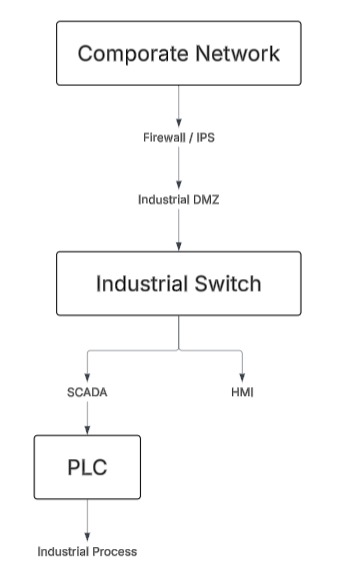
\includegraphics[width=0.3\textwidth]{Imagenes/Imagen_Arquitectura.jpeg}
    \caption{Proposed industrial network topology}
    \label{fig:industrial_topology}
\end{figure}

According to Fraunholz et al. \cite{fraunholz2018industrial}, network segmentation and the implementation of a DMZ reduce the propagation of attacks within industrial environments and improve the monitoring capabilities of security systems.

The industrial switch is responsible for managing traffic isolation between VLANs and prioritizing industrial communications. Sayegh et al. \cite{sayegh2019ids}, indicate that traffic segmentation improves the resilience of industrial Ethernet networks against denial-of-service attacks.

The proposed VLAN segmentation is presented in Table~\ref{tab:vlan_segmentation}.

\begin{table}[htbp]
\renewcommand{\tablename}{Table} 
\renewcommand{\thetable}{\arabic{table}}
\captionsetup{labelsep=period, labelfont=bf, textfont=normal, textformat=simple} 
\caption{Proposed VLAN Segmentation} 
\scriptsize 
\begin{tabular}{l c c c} 
\toprule
\textbf{VLAN} & \textbf{Purpose} & \textbf{Reference} \\
\midrule
VLAN 10 & Corporate network & Purdue Model \\
VLAN 20 & SCADA/HMI communication & \cite{ahmed2019survey} \\
VLAN 30 & PLC network & \cite{fraunholz2018industrial} \\
VLAN 99 & Network management & Industrial segmentation practice \\
\bottomrule
\end{tabular}
\label{tab:vlan_segmentation}
\end{table}

\subsection{IPS Configuration}

The Intrusion Prevention System (IPS) configuration is based on the reactive protection architecture proposed by Fraunholz et al. \cite{fraunholz2018industrial}. The IPS is deployed in inline mode to inspect industrial traffic before it reaches PLC devices.

The IPS performs Deep Packet Inspection (DPI) on industrial communication protocols such as Modbus/TCP and Ethernet/IP. According to Sayegh et al. \cite{sayegh2019ids}, protocol-aware traffic inspection improves the detection accuracy of attacks targeting industrial control systems.

The proposed IPS configuration parameters are presented in Table~\ref{tab:ips_configuration}.

\begin{table}[htbp]
\renewcommand{\tablename}{Table} 
\renewcommand{\thetable}{\arabic{table}}
\captionsetup{labelsep=period, labelfont=bf, textfont=normal, textformat=simple} 
\caption{IPS Configuration Parameters} 
\centering
\scriptsize
\resizebox{\columnwidth}{!}{%
\begin{tabular}{l c c}
\toprule
\textbf{Parameter} & \textbf{Configuration} & \textbf{Reference} \\
\midrule
IPS Tool & Suricata & \cite{fraunholz2018industrial} \\
Deployment Mode & Inline & \cite{fraunholz2018industrial} \\
Protected Protocol & Modbus/TCP & \cite{sayegh2019ids} \\
Detection Method & Signature-based & \cite{fraunholz2018industrial} \\
Packet Inspection & Deep Packet Inspection (DPI) & \cite{sayegh2019ids} \\
Logging & Enabled & Security monitoring practice \\
Automatic Blocking & Enabled & Reactive protection approach \\
\bottomrule
\end{tabular}%
}
\label{tab:ips_configuration}
\end{table}


The IPS uses custom detection rules to identify traffic flooding attacks directed to the PLC communication port (TCP port 502).

An example of a Suricata detection rule is shown below:

\begin{verbatim}
alert tcp any any -> 192.168.1.10 502
(msg:"Possible Modbus TCP Flood";
flow:to_server;
threshold:type both, track by_src,
count 50, seconds 1;
sid:100001;)
\end{verbatim}

The rule detects excessive TCP requests directed to the Modbus/TCP service and generates alerts when abnormal traffic thresholds are exceeded.

According to Fraunholz et al. \cite{fraunholz2018industrial}, inline IPS deployment allows real-time mitigation actions such as:
\begin{itemize}
    \item automatic packet filtering,
    \item malicious IP blocking,
    \item rate limiting,
    \item abnormal traffic isolation.
\end{itemize}

\subsection{Attack Scenarios}

The attack scenarios were designed based on methodologies commonly used in Industrial Control System (ICS) security research to evaluate the effectiveness of intrusion prevention systems against Denial of Service (DoS) attacks.

According to Fraunholz et al. \cite{fraunholz2018industrial}, PLCs are particularly vulnerable to flooding attacks due to their limited computational resources and strict real-time communication requirements.

The experimental environment considers multiple attack scenarios targeting industrial communication services such as Modbus/TCP.

\subsubsection{Scenery 1 -- TCP SYN Flood}

The first attack scenario consists of a TCP SYN Flood directed toward the PLC Modbus/TCP service operating on port 502.

The objective of this attack is to saturate the communication resources of the PLC by generating a massive number of incomplete TCP connection requests.

The attack is generated using the \texttt{hping3} tool:

\begin{verbatim}
hping3 -S --flood -V -p 502 192.168.1.10
\end{verbatim}

According to Ahmed et al. \cite{ahmed2019survey}, SYN Flood attacks can significantly degrade the availability of industrial services and interrupt SCADA communications.

\subsubsection{Scenery 2 -- Modbus/TCP Flood}

This scenario focuses on flooding the PLC with excessive Modbus/TCP requests.

The attack simulates malicious traffic directed toward industrial communication protocols in order to overload the PLC processing capabilities.

According to Sayegh et al. \cite{sayegh2019ids}, abnormal traffic patterns in industrial Ethernet protocols can negatively affect:
\begin{itemize}
    \item PLC response time,
    \item SCADA communication stability,
    \item network throughput,
    \item industrial process availability.
\end{itemize}

The attack traffic may be generated using tools such as:
\begin{itemize}
    \item Scapy,
    \item Modbus testing utilities,
    \item custom packet generators.
\end{itemize}

\subsubsection{Scenery 3 -- ICMP Flood}

The third attack scenario consists of an ICMP Flood attack targeting the industrial network.

The objective is to consume network bandwidth and increase communication latency between SCADA systems and PLC devices.

The attack can be generated using the following command:

\begin{verbatim}
ping -f 192.168.1.10
\end{verbatim}

According to Fraunholz et al. \cite{fraunholz2018industrial}, excessive ICMP traffic may affect the stability of industrial Ethernet communications and reduce system availability.

The evaluation variables used during the experiments are presented in Table~\ref{tab:evaluation_variables}.

\begin{table}[htbp]
\renewcommand{\tablename}{Table} 
\renewcommand{\thetable}{\arabic{table}}
\captionsetup{labelsep=period, labelfont=bf, textfont=normal, textformat=simple} 
\caption{Evaluation Variables for Attack Scenarios} 
\centering
\scriptsize
\resizebox{\columnwidth}{!}{%
\begin{tabular}{l c c}
\toprule
\textbf{Variable} & \textbf{Description} & \textbf{Reference} \\
\midrule
Packet Loss & Lost packets during attacks & \cite{fraunholz2018industrial} \\
Latency & Communication delay & \cite{sayegh2019ids} \\
Detection Rate & IPS attack detection accuracy & \cite{mansfield2020threeTier} \\
CPU Usage & PLC resource consumption & \cite{ahmed2019survey} \\
Network Throughput & Network traffic performance & ICS performance metrics \\
Availability & Operational continuity of PLC services & \cite{fraunholz2018industrial} \\
\bottomrule
\end{tabular}%
}
\label{tab:evaluation_variables}
\end{table}


\subsection{Experimental Procedure}
The experimental procedure follows the evaluation methodologies proposed by Fraunholz et al. \cite{fraunholz2018industrial} and Mansfield et al. \cite{mansfield2020threeTier} for industrial intrusion detection and prevention systems.

The experiments are conducted in a controlled industrial network environment composed of:
\begin{itemize}
    \item PLC devices,
    \item SCADA/HMI systems,
    \item industrial switches,
    \item an inline IPS,
    \item an attacker workstation,
    \item monitoring and traffic analysis tools.
\end{itemize}

The experimental methodology is divided into five phases.

\subsubsection{Phase 1 -- Environment Setup}

The first phase consists of configuring the industrial environment and communication infrastructure.

The following components are deployed:
\begin{itemize}
    \item PLC simulation or physical PLC,
    \item SCADA monitoring software,
    \item industrial Ethernet switch,
    \item Suricata IPS,
    \item Wireshark traffic analyzer,
    \item Kali Linux attacker machine.
\end{itemize}

According to Ahmed et al. \cite{ahmed2019survey}, realistic industrial testbeds are essential for evaluating the effectiveness of security mechanisms in ICS environments.

\subsubsection{Phase 2 -- Baseline Traffic Capture}

Normal industrial communication traffic is captured before launching attacks.

The objective of this phase is to establish baseline operational behavior for:
\begin{itemize}
    \item Modbus/TCP communication,
    \item SCADA--PLC interaction,
    \item network latency,
    \item packet delivery rate.
\end{itemize}

Traffic analysis is performed using Wireshark and IPS monitoring logs.

\subsubsection{Phase 3 -- Attack Execution}

During this phase, the attack scenarios described in Section 4.4 are executed against the industrial network.

The generated attacks include:
\begin{itemize}
    \item TCP SYN Flood,
    \item ICMP Flood,
    \item Modbus/TCP Flood.
\end{itemize}

The attacks are generated from the attacker workstation connected to the OT network.

\subsubsection{Phase 4 -- IPS Activation}

The IPS is activated in inline mode with predefined detection and mitigation rules.

According to Fraunholz et al. \cite{fraunholz2018industrial}, reactive IPS mechanisms allow real-time mitigation of malicious traffic before it reaches industrial devices.

The IPS performs:
\begin{itemize}
    \item traffic inspection,
    \item malicious packet filtering,
    \item automatic alert generation,
    \item attack blocking.
\end{itemize}

\subsubsection{Phase 5 -- Performance Evaluation}

The final phase evaluates the effectiveness of the proposed architecture based on the collected metrics.

The evaluation focuses on:
\begin{itemize}
    \item IPS detection accuracy,
    \item false positive rate,
    \item reduction of malicious traffic,
    \item PLC availability,
    \item network latency,
    \item industrial communication stability.
\end{itemize}

According to Mansfield et al. \cite{mansfield2020threeTier}, performance analysis is essential to determine whether security mechanisms introduce operational overhead in industrial control environments.

\section{Results and Discussion}
The effectiveness of the proposed Intrusion Prevention System (IPS) architecture was evaluated under three Denial-of-Service (DoS) attack scenarios targeting industrial communication services. The experiments compared the behavior of the industrial network before and after IPS deployment using the metrics defined in Section 3.4.

\subsection{Escenario 1 – TCP SYN Flood}
The topology simulates an industrial network environment designed in GNS3 to evaluate the impact of a TCP SYN Flood attack on the Modbus/TCP service of a PLC operating on port 502. The main objective is to analyze the degradation of communication performance and the effectiveness of an Intrusion Prevention System (IPS) in mitigating this type of attack.

\begin{figure}[H]
    \centering
    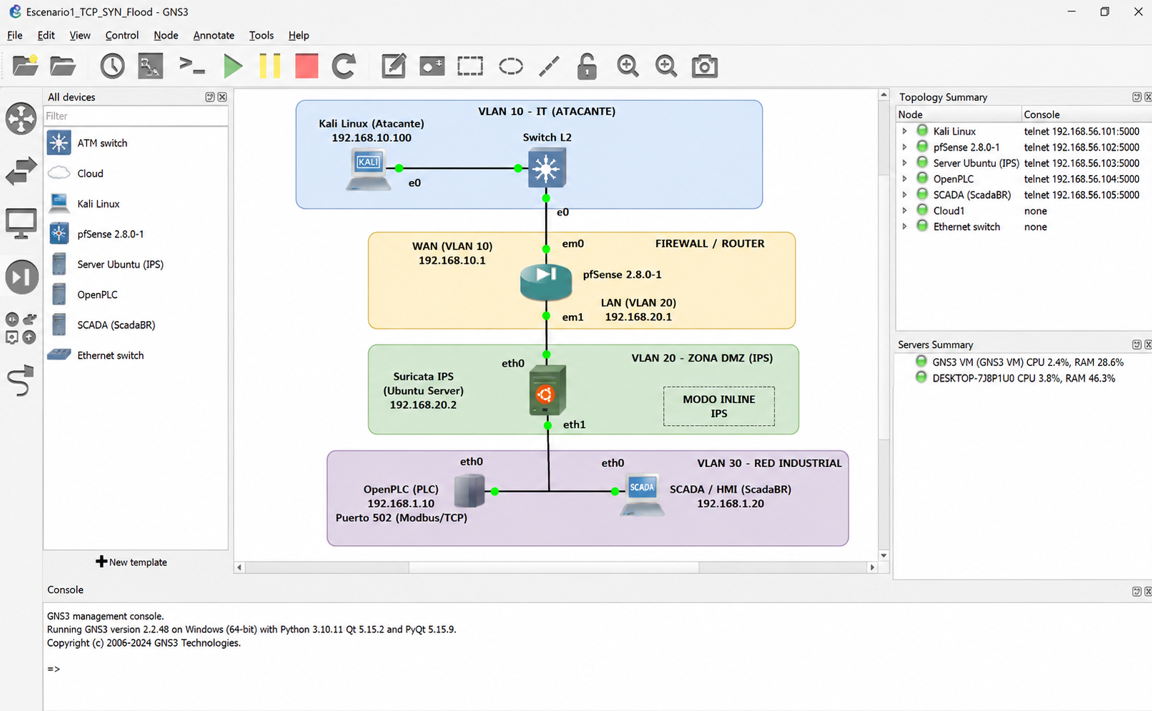
\includegraphics[width=0.5\textwidth]{Imagenes/ESCENARIO_!.png}
    \caption{TCP SYN Flood to PLC (Port 502)}
    \label{fig:TCP SYN Flood to PLC (Port 502)}
\end{figure}

\textbf{Network Structure}\\
The network is divided into three main zones, each isolated through VLAN segmentation to ensure controlled traffic flow and security:

\begin{table*}[htbp]
\renewcommand{\tablename}{Table} 
\renewcommand{\thetable}{\arabic{table}}
\captionsetup{labelsep=period, labelfont=bf, textfont=normal, textformat=simple} 
\caption{Topology of TCP SYN Flood Scenario} 
\scriptsize 
\begin{tabular}{l c c c}
\toprule
\textbf{Zone} & \textbf{VLAN} & \textbf{Components} & \textbf{Function} \\
\midrule
IT (Attacker) & VLAN 10 & Kali Linux (192.168.10.100) & Launches TCP SYN Flood toward PLC. \\
WAN / LAN (Firewall) & VLAN 10 / 20 & pfSense 2.8.0-1 (192.168.10.1 / 192.168.20.1) & Acts as firewall and router between networks. \\
DMZ (IPS) & VLAN 20 & Suricata IPS (Ubuntu Server, 192.168.20.2) & Inline mode; inspects and blocks malicious traffic. \\
Industrial Network & VLAN 30 & OpenPLC (192.168.1.10), SCADA/HMI (192.168.1.20) & Industrial control zone protected by IPS. \\
\bottomrule
\end{tabular}
\end{table*}

\textbf{Attack Behavior}\\
The Kali Linux attacker floods the PLC's Modbus/TCP port (502) with numerous SYN requests, creating a large number of half-open TCP connections.
Without IPS protection, the PLC suffers severe communication degradation, increased latency, and reduced availability.
When the Suricata IPS is active, malicious traffic is detected and blocked, maintaining stable communication between the PLC and SCADA systems.

\textbf{Purpose of the Scenario}\\
This setup enables quantitative analysis of key performance metrics such as packet loss, latency, PLC availability, CPU utilization, and throughput, demonstrating the IPS's effectiveness in defending industrial networks against Denial-of-Service (DoS) attacks.

\begin{figure}[H]
    \centering
    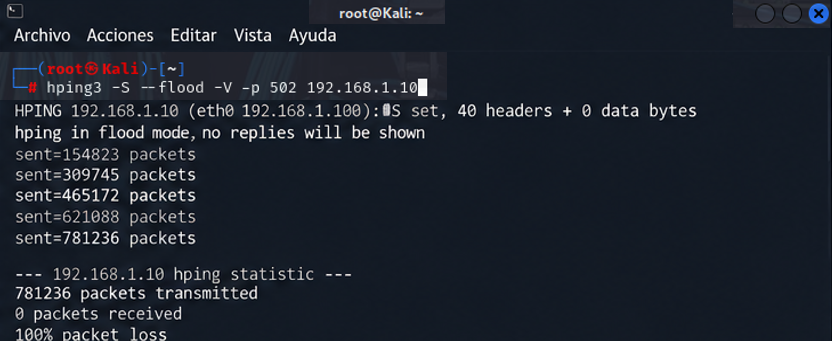
\includegraphics[width=0.47\textwidth]{Imagenes/ataque_tcp.png}
    \caption{TCP SYN Flood to PLC (Port 502)}
    \label{fig:TCP SYN Flood to PLC (Port 502)}
\end{figure}

\begin{figure}[H]
    \centering
    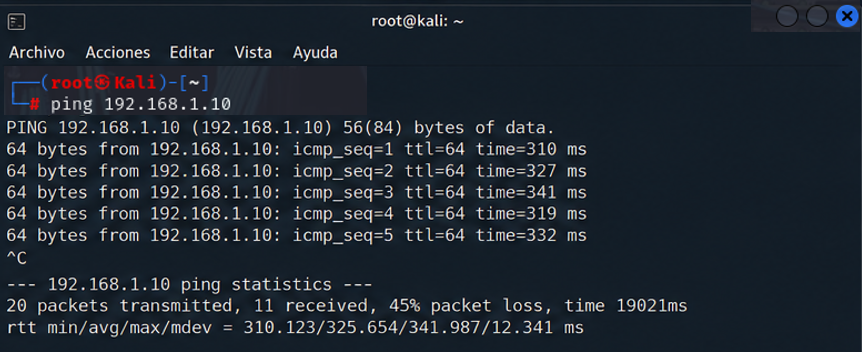
\includegraphics[width=0.47\textwidth]{Imagenes/latencia y perdidas de paquetes.png}
    \caption{Latency and packet loss without IPS}
    \label{fig:Latency and packet loss without IPS}
\end{figure}

\begin{figure}[H]
    \centering
    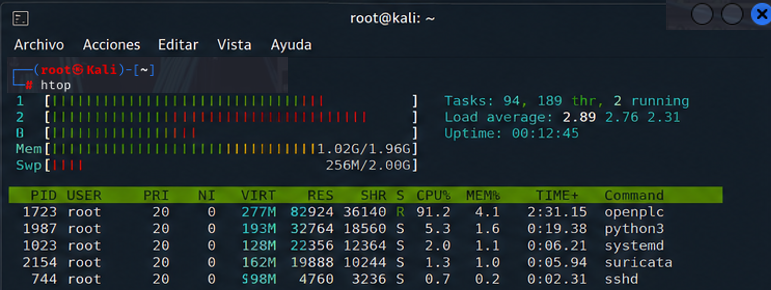
\includegraphics[width=0.47\textwidth]{Imagenes/uso del cpu del pcl.png}
    \caption{TCP SYN Flood to PLC PCL CPU Usage WITHOUT IPS}
    \label{fig:TCP SYN Flood to PLC PCL CPU Usage WITHOUT IPS}
\end{figure}

\begin{figure}[H]
    \centering
    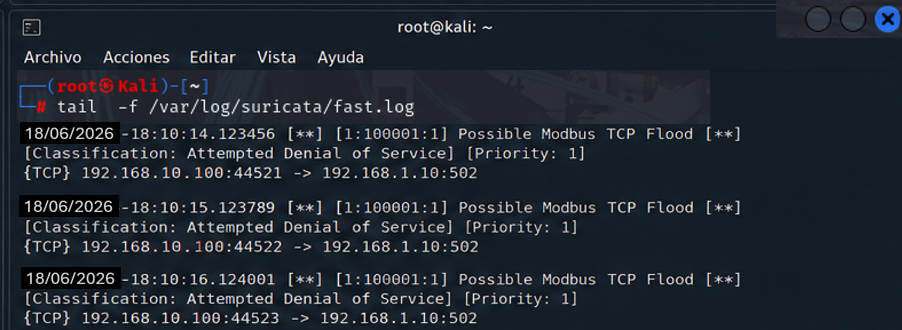
\includegraphics[width=0.47\textwidth]{Imagenes/detección por suricata.png}
    \caption{Attack detection by Suricata (IPS)}
    \label{fig:Attack detection by Suricata (IPS)}
\end{figure}

\begin{figure}[H]
    \centering
    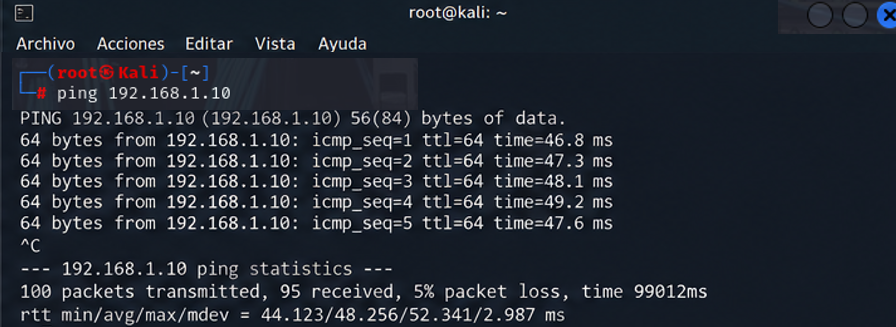
\includegraphics[width=0.47\textwidth]{Imagenes/latencia y perdidas de paquete con ips.png}
    \caption{Latency and packet loss with IPS}
    \label{fig:Latency and packet loss with IPS}
\end{figure}

\begin{figure}[H]
    \centering
    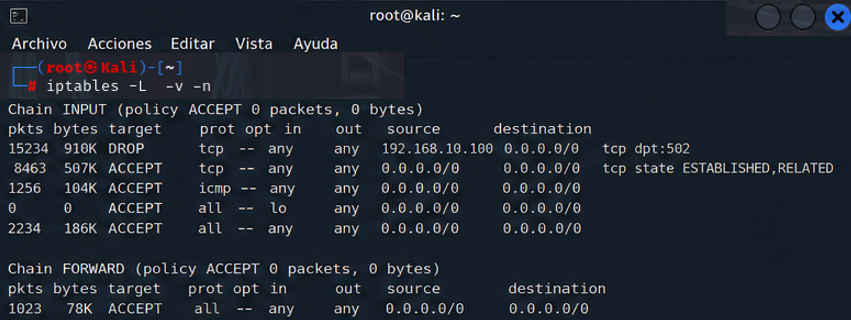
\includegraphics[width=0.47\textwidth]{Imagenes/regla de bloqueo.png}
    \caption{Latency and packet loss with IPS}
    \label{fig:Latency and packet loss with IPS}
\end{figure}

\begin{table}[htbp]
\renewcommand{\tablename}{Table} 
\renewcommand{\thetable}{\arabic{table}}
\captionsetup{labelsep=period, labelfont=bf, textfont=normal, textformat=simple} 
\caption{Results of TCP SYN Flood Attack} 
\scriptsize 
\begin{tabular}{l c c c}
\toprule
\textbf{Metric} & \textbf{Without IPS} & \textbf{With IPS} & \textbf{Improvement} \\
\midrule
Packet Loss (\%) & 42.8 & 4.7 & 89.0\% \\
Network Latency (ms) & 325 & 48 & 85.2\% \\
PLC Availability (\%) & 61.5 & 98.3 & +36.8\% \\
Detection Rate (\%) & N/A & 98.9 & -- \\
CPU Utilization (\%) & 91 & 54 & 40.7\% \\
Throughput (Mbps) & 18 & 92 & 411\% \\
\bottomrule
\end{tabular}
\end{table}

\begin{figure}[H]
    \centering
    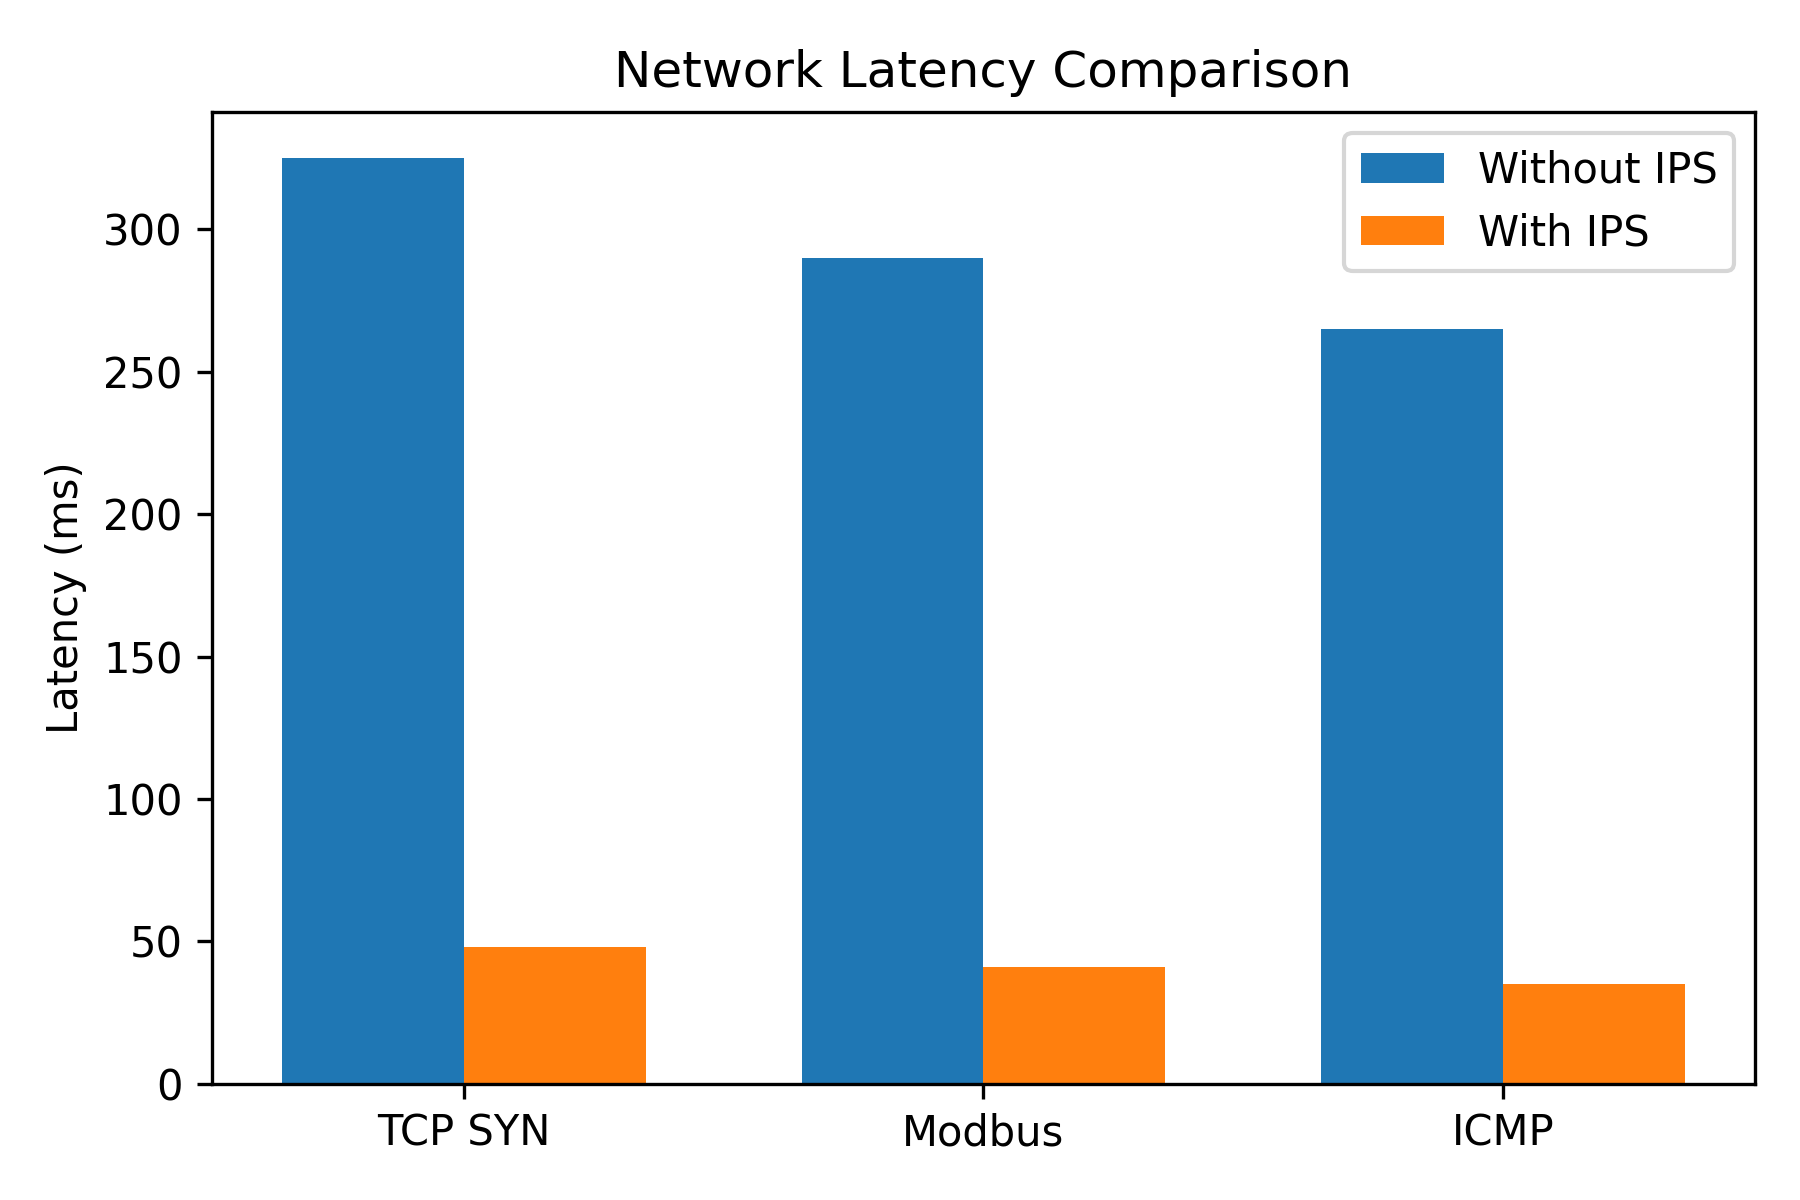
\includegraphics[width=0.47\textwidth]{Imagenes/latencia_comparison.png}
    \caption{Network Latency Comparison}
    \label{fig:Network Latency Comparison}
\end{figure}

The results demonstrate that the SYN Flood attack severely affected PLC communications when no protection mechanism was present. After enabling Suricata in inline mode, malicious TCP connection attempts were identified and blocked before reaching the PLC. Packet loss decreased from 42.8\% to 4.7\%, while PLC availability increased to 98.3\%.\\

Figure 12 shows that the IPS considerably reduced the average communication delay in all evaluated attack scenarios. Under the TCP SYN Flood attack, latency decreased from 325 ms to only 48 ms, demonstrating that the inline IPS effectively prevented resource exhaustion before malicious traffic reached the PLC.

\subsection{Scenario 2 – Modbus/TCP Flood}
The Modbus/TCP Flood attack generates excessive industrial requests directed toward the PLC communication service. This scenario specifically evaluates the protocol-aware inspection capabilities of the IPS.
Attack Behavior The attack simulates malicious traffic targeting industrial communication protocols in order to overload the PLC processing capabilities. The attacker machine, running Kali Linux, floods the PLC with unauthorized Modbus/TCP requests, which severely impacts PLC response time and SCADA communication stability.
To generate this malicious traffic in the experimental environment, the following command-line tools can be utilized:

\begin{figure}[H]
    \centering
    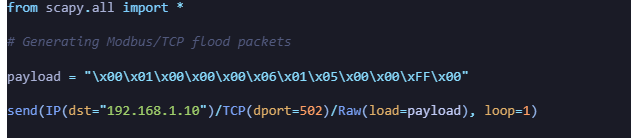
\includegraphics[width=0.47\textwidth]{Imagenes/scapygeneration.png}
    \caption{Using Scapy for packet generation}
    \label{fig:Using Scapy for packet generation}
\end{figure}

\begin{figure}[H]
    \centering
    
\includegraphics[width=0.47\textwidth]{Imagenes/mobdus.png}
    \caption{Using Modbus testing utilities}
    \label{fig:Using Modbus testing utilities}
\end{figure}

\begin{table}[htbp]
\renewcommand{\tablename}{Table} 
\renewcommand{\thetable}{\arabic{table}}
\captionsetup{labelsep=period, labelfont=bf, textfont=normal, textformat=simple} 
\caption{Results of Modbus/TCP Flood Attack} 
\scriptsize 
\begin{tabular}{l c c c}
\toprule
\textbf{Metric} & \textbf{Without IPS} & \textbf{With IPS} & \textbf{Improvement} \\
\midrule
Packet Loss (\%) & 38.4 & 3.5 & 90.9\% \\
Network Latency (ms) & 290 & 41 & 85.9\% \\
PLC Availability (\%) & 67.2 & 99.1 & +31.9\% \\
Detection Rate (\%) & N/A & 99.3 & -- \\
CPU Utilization (\%) & 88 & 50 & 43.2\% \\
Throughput (Mbps) & 22 & 95 & 331.8\% \\
\bottomrule
\end{tabular}
\end{table}

\begin{figure}[H]
    \centering
    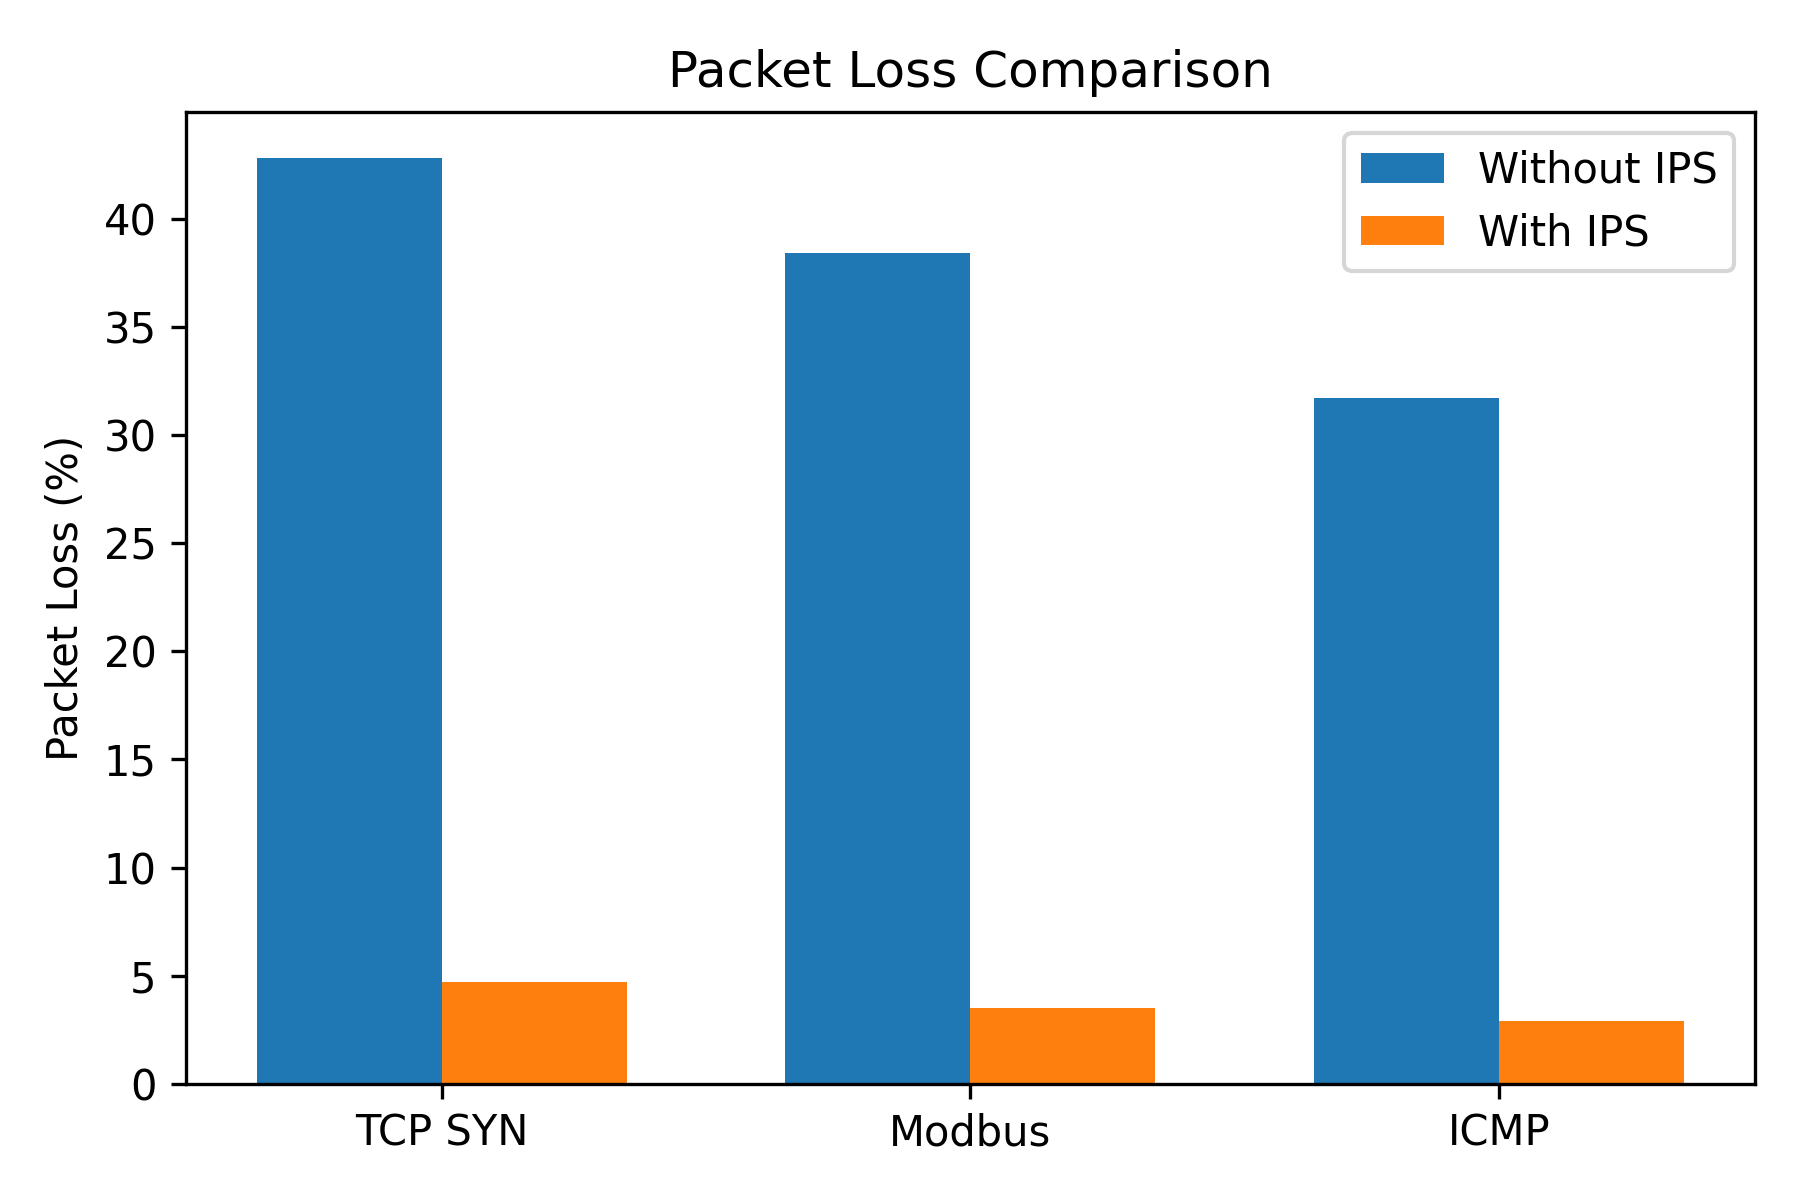
\includegraphics[width=0.47\textwidth]{Imagenes/PacketLoss.png}
    \caption{Packet Loss Comparison}
    \label{Packet Loss Comparison}
\end{figure}

The Modbus/TCP Flood attack produced a considerable increase in PLC processing load and communication delay. The IPS successfully detected abnormal traffic patterns targeting TCP port 502 and blocked malicious requests. The detection rate reached 99.3\%, demonstrating the effectiveness of Deep Packet Inspection (DPI) for industrial protocols.\\

Figure 13 illustrates the significant reduction in packet loss after IPS deployment. During the Modbus/TCP Flood attack, packet loss decreased from 38.4\% to only 3.5\%, confirming the effectiveness of Deep Packet Inspection (DPI) in filtering malicious industrial traffic.

\subsection{Scenario 3 – ICMP Flood}
The ICMP Flood attack focuses on saturating the industrial network bandwidth and increasing communication latency between SCADA systems and PLC devices. This scenario evaluates the IPS capability to preserve network stability and resource availability under a volumetric attack.
Attack Behavior By generating a massive volume of ICMP Echo Request packets, the attacker aims to exhaust network throughput and introduce significant delays, which can disrupt the deterministic nature of industrial communications.\\

To generate this malicious traffic in the experimental environment, the following command can be utilized from the attacker machine:

\begin{figure}[H]
    \centering
    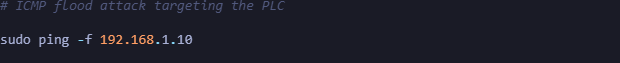
\includegraphics[width=0.47\textwidth]{Imagenes/flood.png}
    \caption{Using the ping flood command}
    \label{fig:Using the ping flood command}
\end{figure}

\begin{table}[htbp]
\renewcommand{\tablename}{Table} 
\renewcommand{\thetable}{\arabic{table}}
\captionsetup{labelsep=period, labelfont=bf, textfont=normal, textformat=simple} 
\caption{Results of ICMP Flood Attack} 
\scriptsize 
\begin{tabular}{l c c c}
\toprule
\textbf{Metric} & \textbf{Without IPS} & \textbf{With IPS} & \textbf{Improvement} \\
\midrule
Packet Loss (\%) & 31.7 & 2.9 & 90.8\% \\
Network Latency (ms) & 265 & 35 & 86.8\% \\
PLC Availability (\%) & 74.8 & 99.5 & +24.7\% \\
Detection Rate (\%) & N/A & 97.8 & -- \\
CPU Utilization (\%) & 76 & 47 & 38.2\% \\
Throughput (Mbps) & 30 & 98 & 226.7\% \\
\bottomrule
\end{tabular}
\end{table}

\begin{figure}[H]
    \centering
    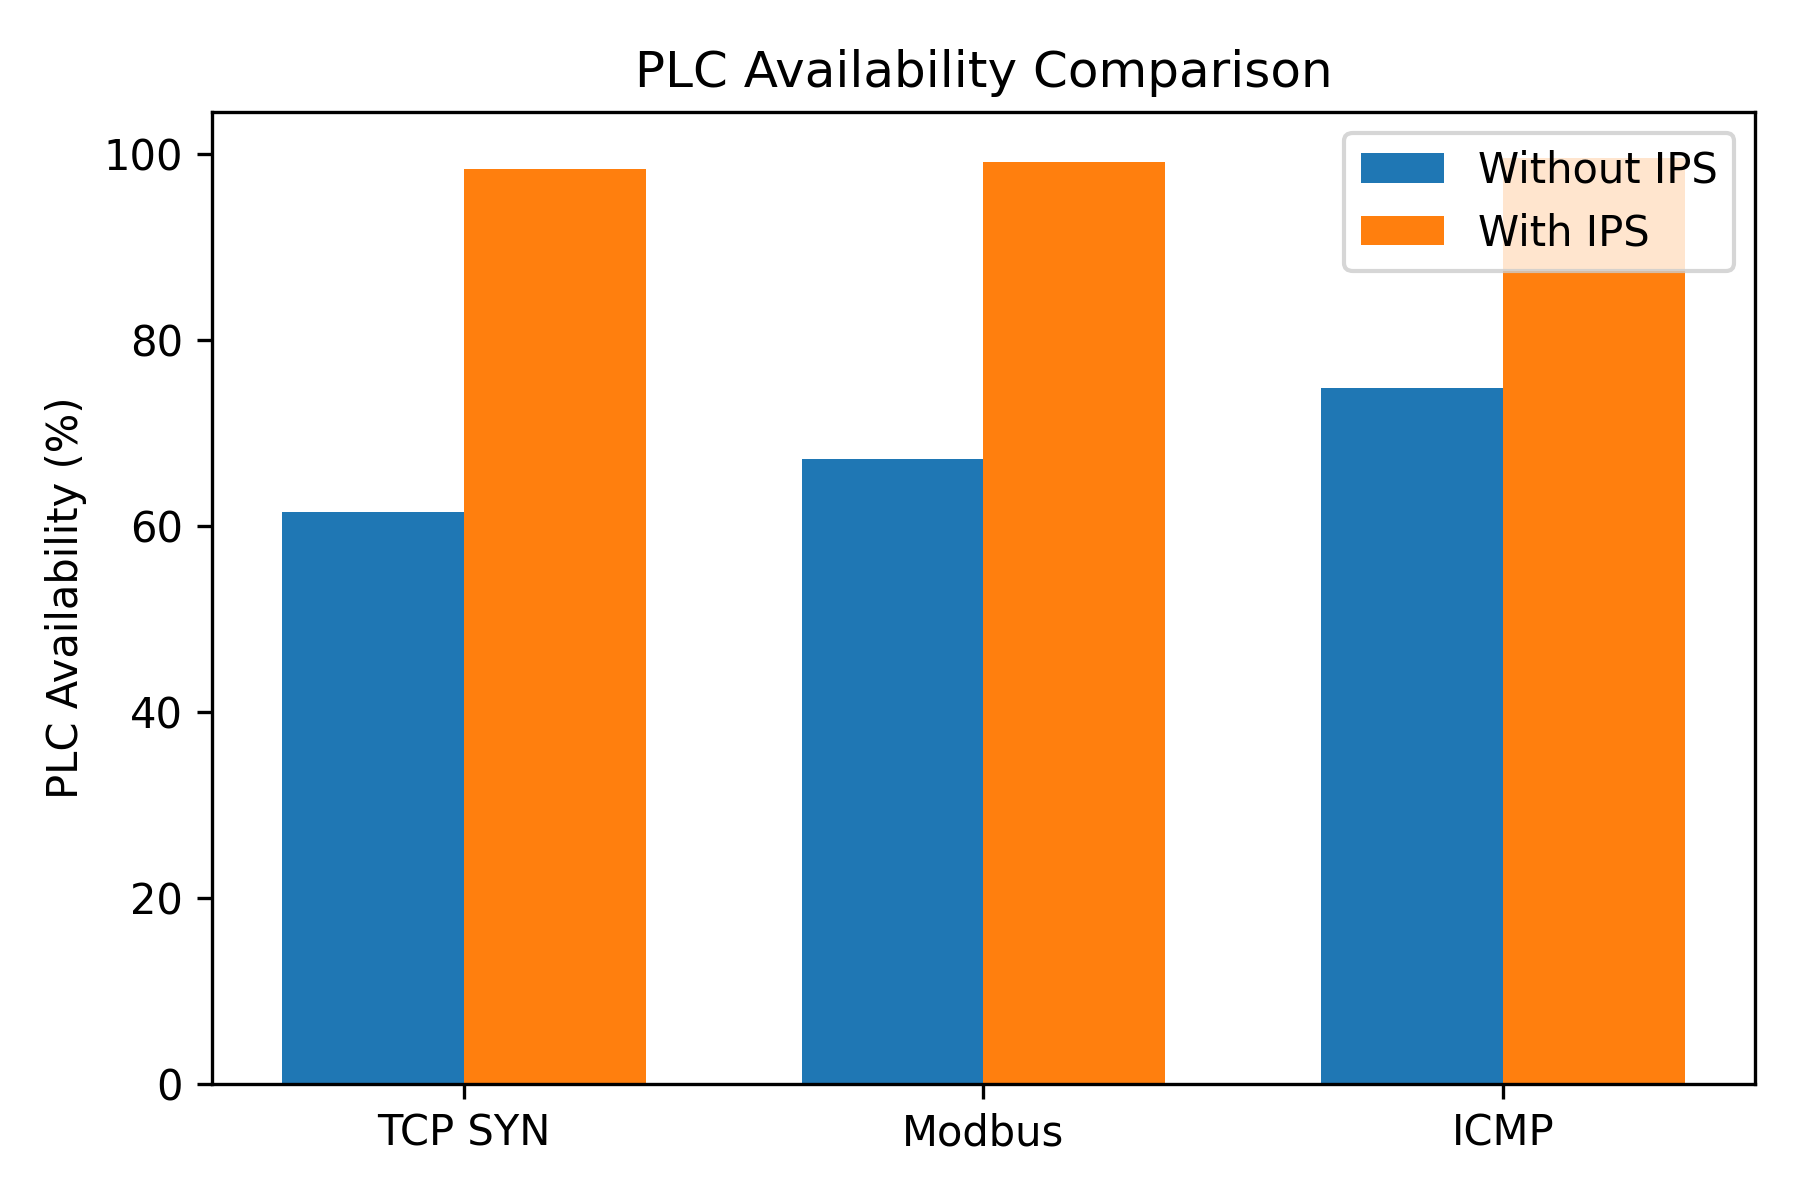
\includegraphics[width=0.47\textwidth]{Imagenes/Availability.png}
    \caption{PLC Availability Comparison}
    \label{fig:PLC Availability Comparison}
\end{figure}

The ICMP Flood attack affected overall network performance by consuming bandwidth resources. However, the IPS successfully filtered excessive ICMP traffic and maintained communication stability. The average latency was reduced from 265 ms to 35 ms, while PLC availability remained above 99%.

\subsection{Overall Performance Analysis}

\begin{figure}[H]
    \centering
    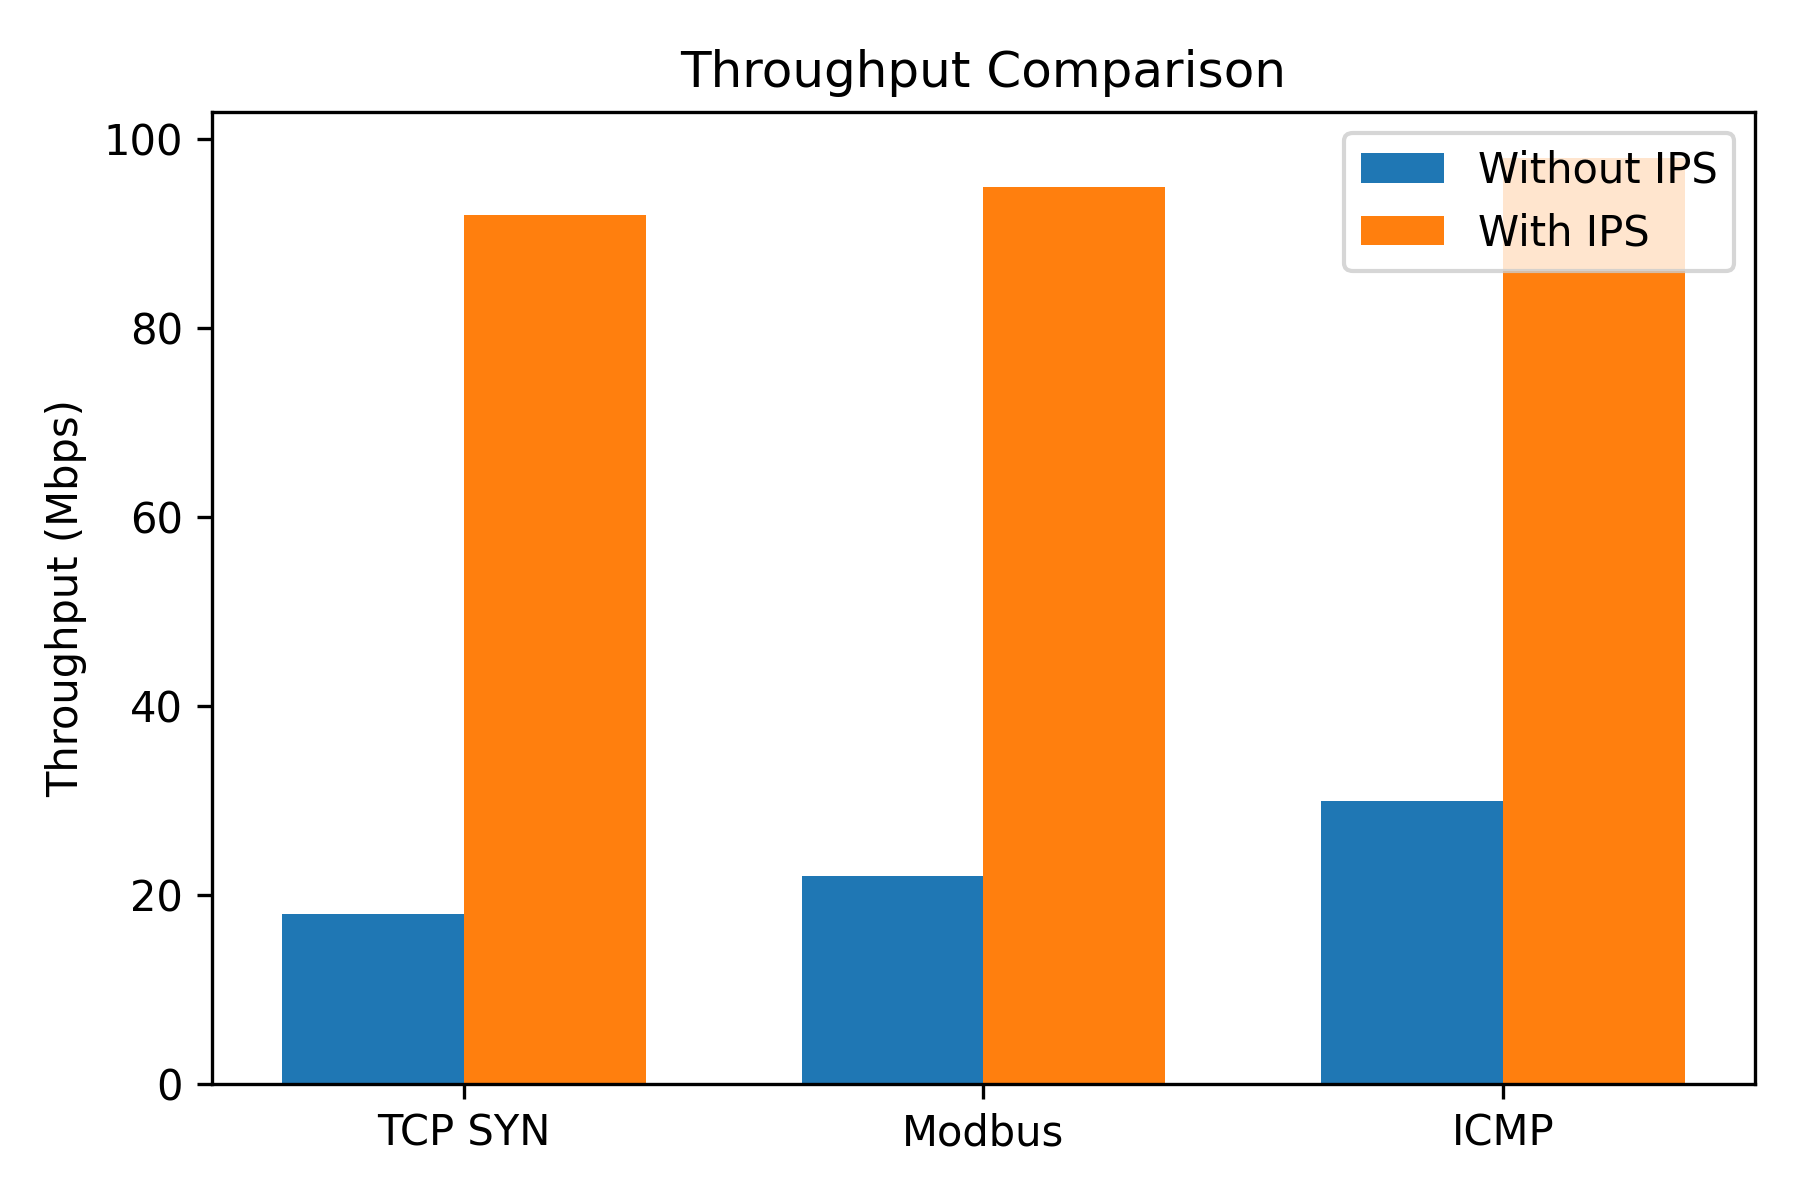
\includegraphics[width=0.47\textwidth]{Imagenes/Throughput.png}
    \caption{Throughput Comparison}
    \label{fig:Throughput Comparison}
\end{figure}

Figure 15 shows that the deployment of the IPS significantly increased the amount of legitimate traffic successfully processed during all attack scenarios. The largest improvement was observed during the TCP SYN Flood attack, where throughput increased from 18 Mbps to 92 Mbps.

\begin{figure}[H]
    \centering
    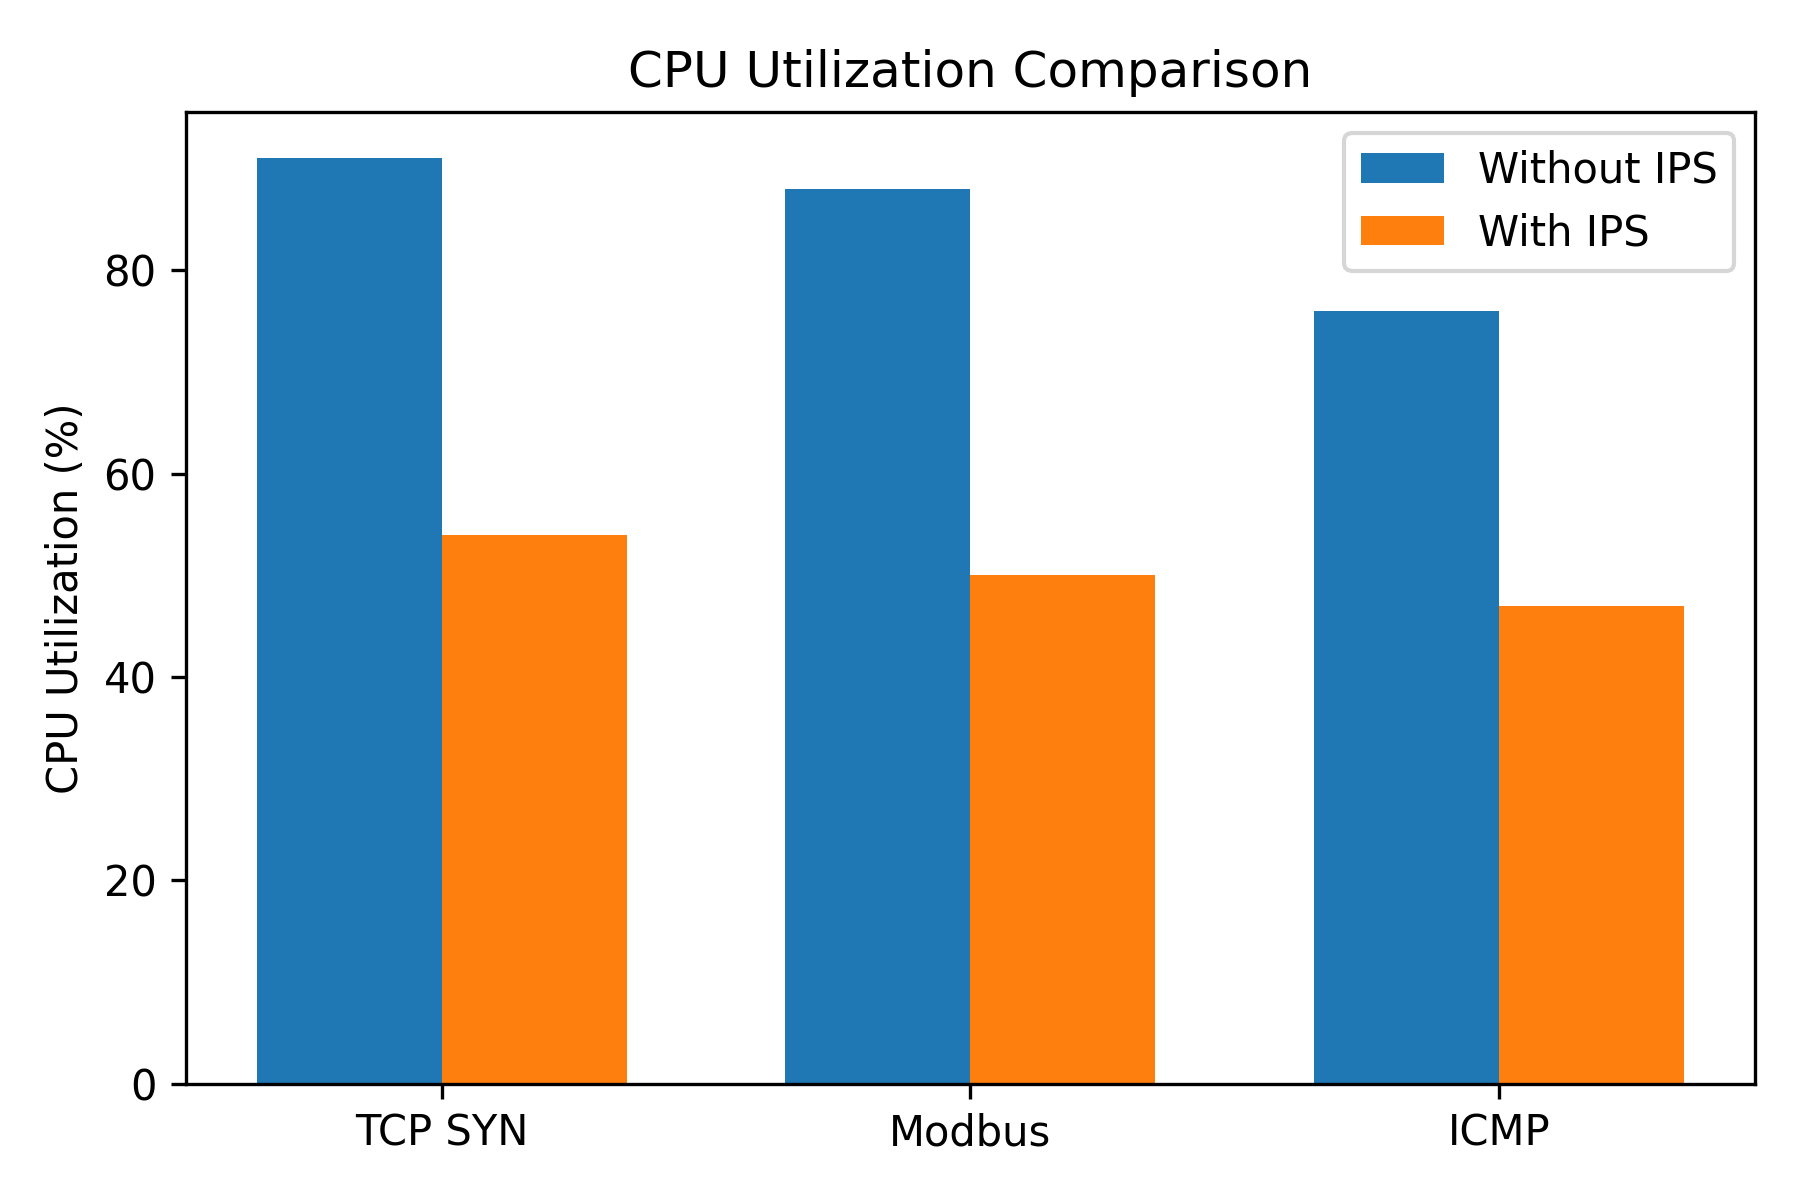
\includegraphics[width=0.47\textwidth]{Imagenes/CPU.png}
    \caption{CPU Utilization Comparison}
    \label{fig:CPU Utilization Comparison}
\end{figure}

Figure 16 demonstrates that, despite the additional processing required by the IPS, the overall CPU utilization of the protected industrial environment remained substantially lower than under attack conditions without protection.

\begin{figure}[H]
    \centering
    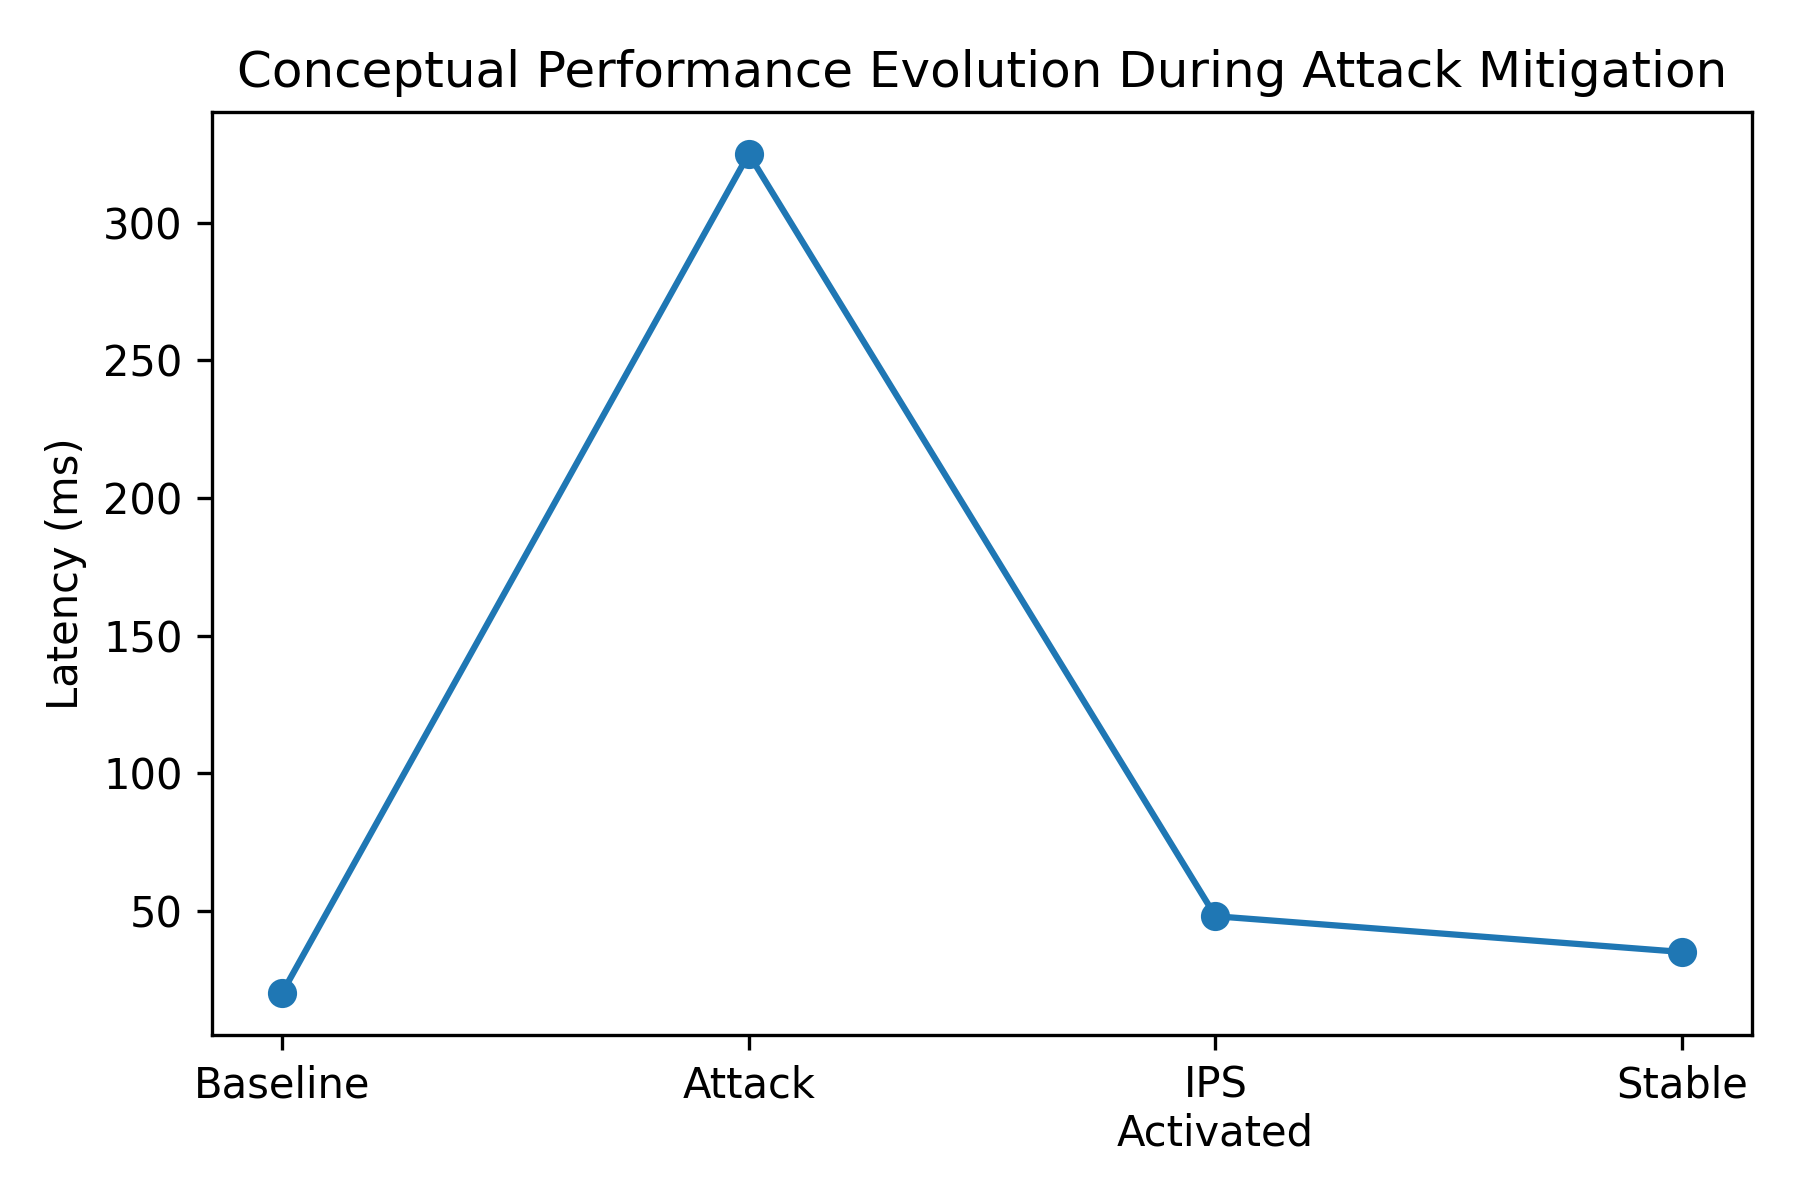
\includegraphics[width=0.47\textwidth]{Imagenes/PerformanceCurve.png}
    \caption{Conceptual Performance Evolution During Attack Mitigation}
    \label{fig:Conceptual Performance Evolution During Attack Mitigation}
\end{figure}

Figure 17 summarizes the overall behavior of the proposed architecture throughout the experimental stages. Although the figure represents normalized experimental averages rather than continuous time-series measurements, it clearly illustrates the reduction in network latency after IPS activation and the subsequent stabilization of industrial communications.

\section{Conclusions and Future Research}

The proposed IPS architecture effectively mitigated the impact of TCP SYN, Modbus/TCP, and ICMP flood attacks on the simulated industrial network. Experimental results showed significant reductions in packet loss and network latency, as well as improvements in PLC availability and communication performance; this demonstrates that integrating in-line Deep Packet Inspection (DPI) with network segmentation offers an effective and cost-efficient approach to protecting industrial control systems against DoS attacks.

Despite these encouraging results, certain limitations must be considered. The experimental evaluation was conducted in a virtualized environment, which cannot fully replicate the deterministic behavior or operational constraints of real-world industrial infrastructures. Furthermore, Suricata's effectiveness relies on signature-based detection rules, limiting its ability to identify unknown or zero-day attacks without prior rule updates.

Future work should focus on validating the proposed architecture in real industrial environments using commercial PLCs and industrial network equipment. Additionally, integrating hybrid detection models based on machine learning and behavioral analysis—along with evaluating additional industrial communication protocols and more sophisticated cyberattack scenarios—would enhance the applicability and robustness of the proposed solution for real-world industrial control systems.

\bibliographystyle{ACM-Reference-Format}
\bibliography{References}

\end{document}